\documentclass[a4paper]{article}
\usepackage[utf8]{inputenc}
\usepackage[russian]{babel}
\usepackage{listings}
\usepackage[a4paper]{geometry}
\usepackage{indentfirst}
\usepackage{graphicx}
\usepackage{caption}
\usepackage{float}

\begin{document}

\title{Лабораторная работа 4 по курсу <<Нелинейная динамика и её приложения>>. \\Отчёт.}
\author{Владислав Соврасов\\ 381503м4}
\date{}
\maketitle

\section{}

\begin{figure}[H]
	\center
	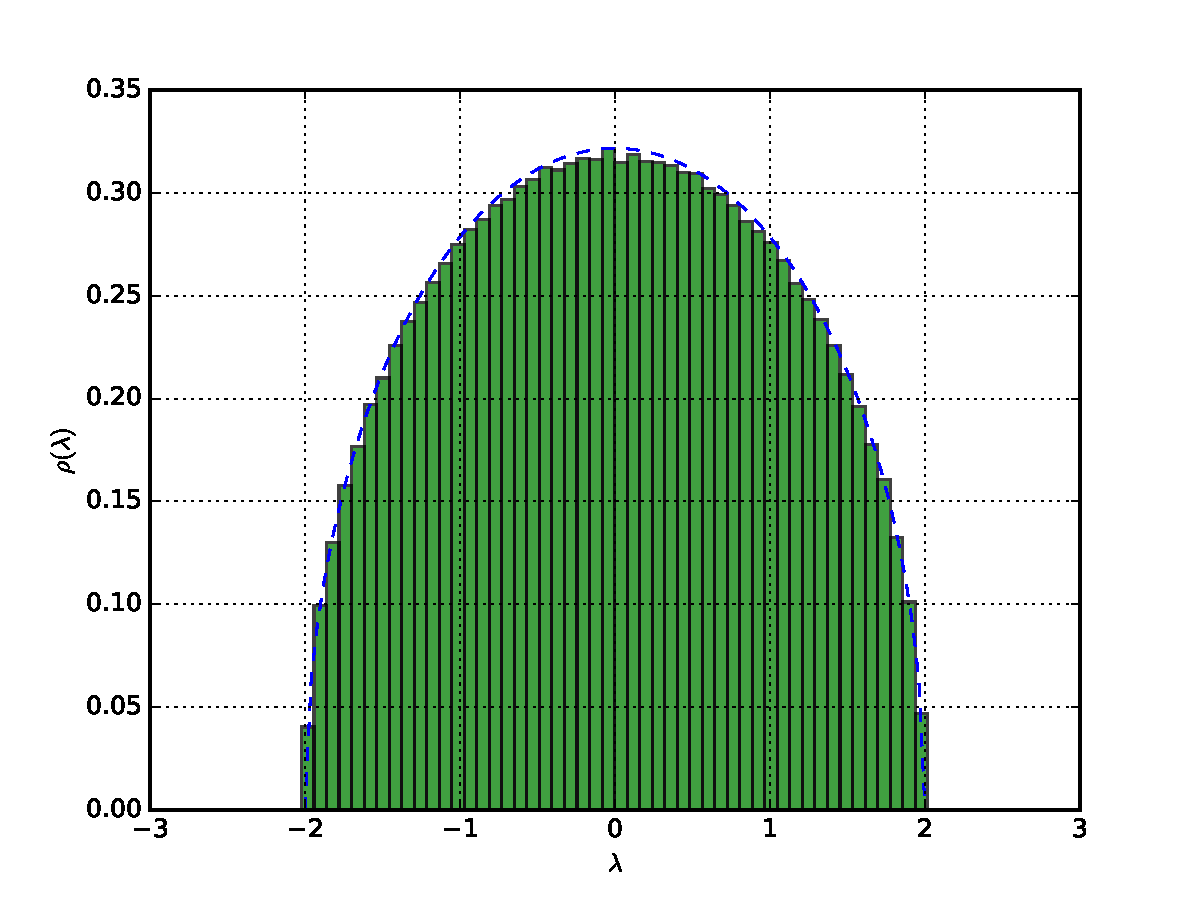
\includegraphics[width=0.75\textwidth]{../pictures/lab4_goe_eig_hist.pdf}
	\caption{Распределение нормированных собственных чисел для GOE}
	\label{fig:goe_eig}
\end{figure}

\begin{figure}[H]
	\center
	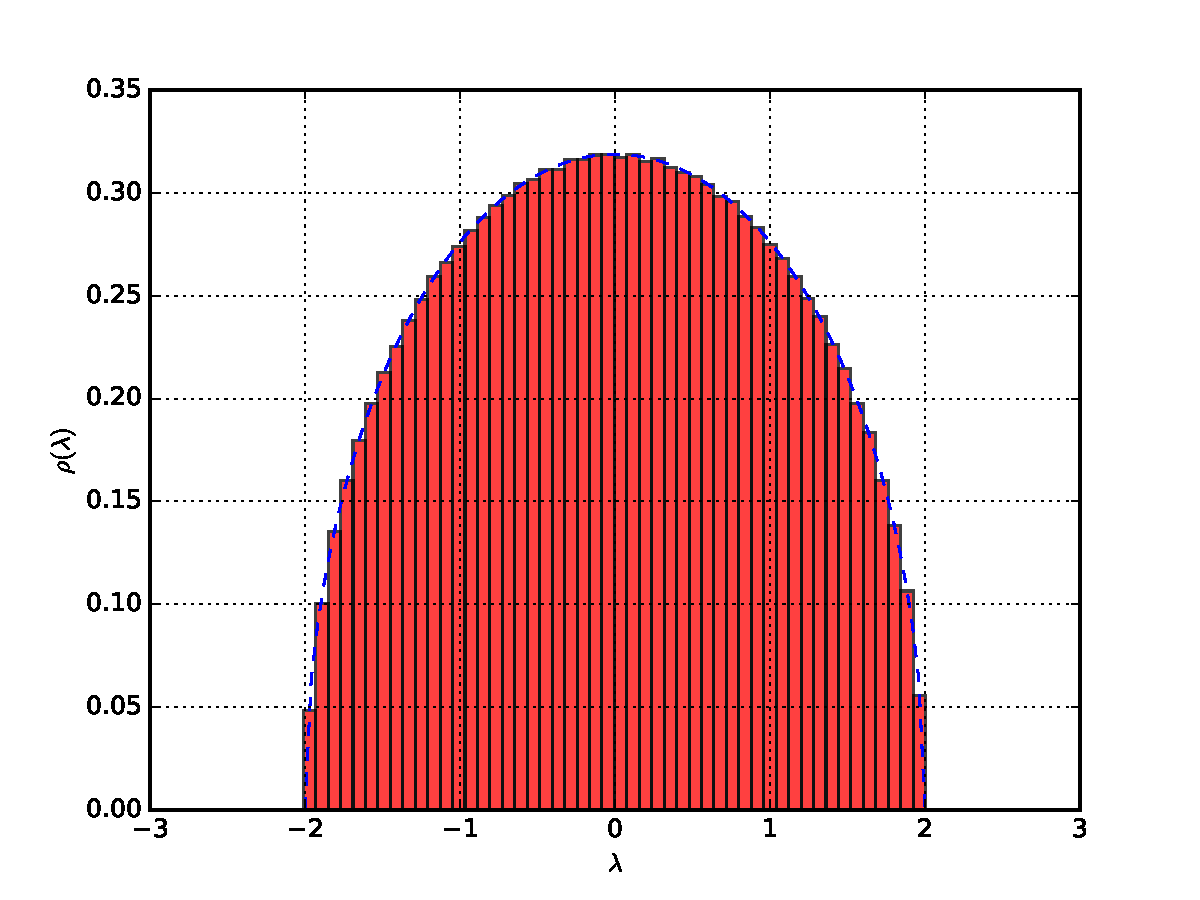
\includegraphics[width=0.75\textwidth]{../pictures/lab4_gue_eig_hist.pdf}
	\caption{Распределение нормированных собственных чисел для GUE}
	\label{fig:gue_eig}
\end{figure}

\begin{figure}[H]
	\center
	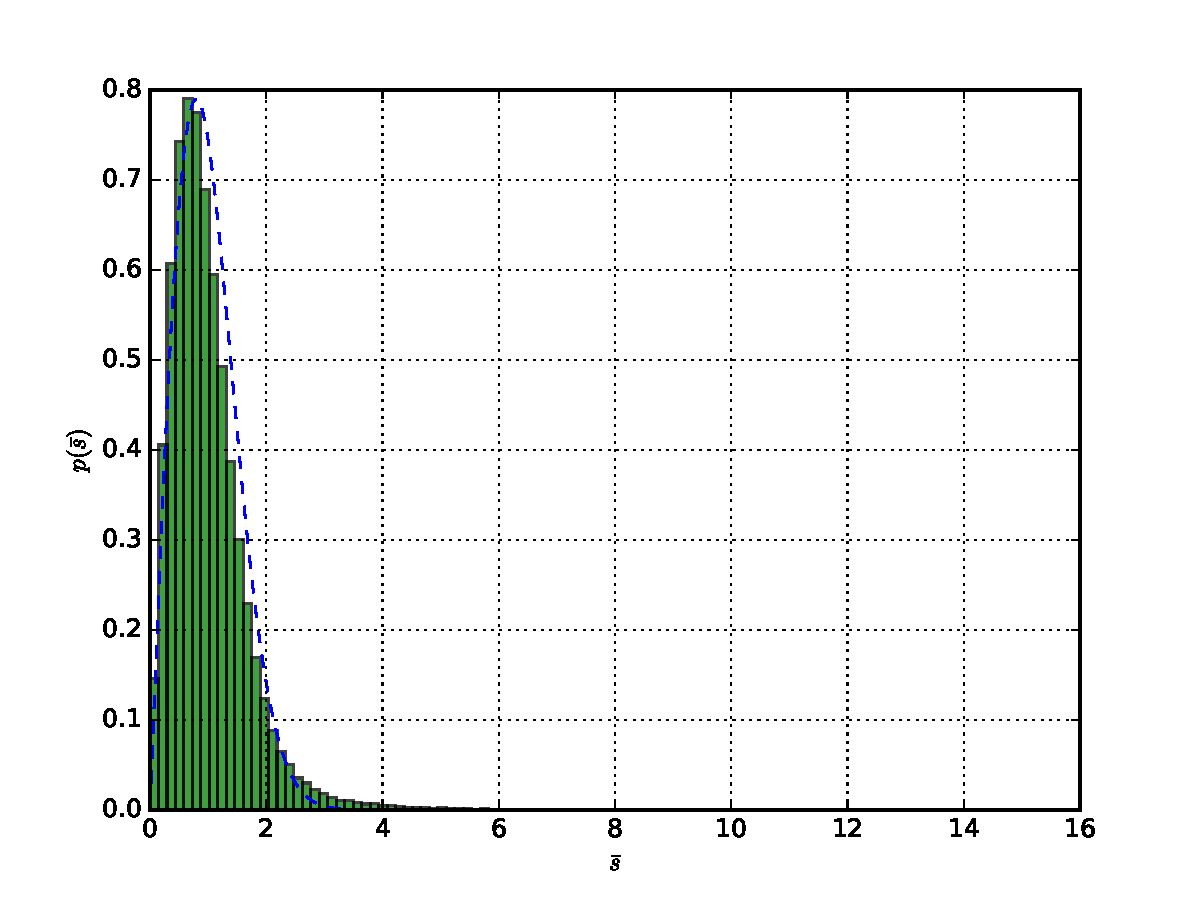
\includegraphics[width=0.75\textwidth]{../pictures/lab4_goe_spacing_hist.pdf}
	\caption{Распределение нормированных расщеплени уровней для GOE}
	\label{fig:goe_spacing}
\end{figure}

\begin{figure}[H]
	\center
	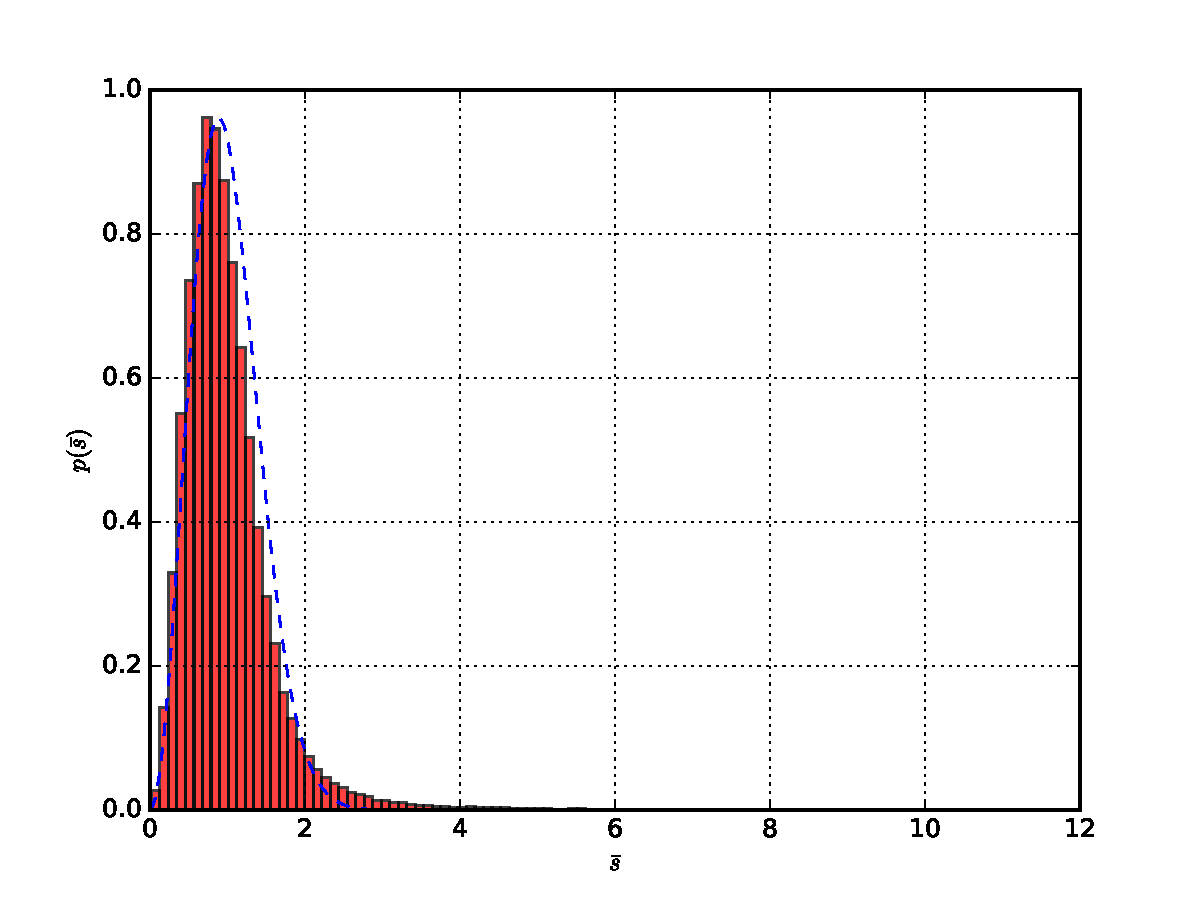
\includegraphics[width=0.75\textwidth]{../pictures/lab4_gue_spacing_hist.pdf}
	\caption{Распределение нормированных расщеплений уровней для GUE}
	\label{fig:gue_spacing}
\end{figure}


\section{Исходный код}
\lstinputlisting[language=Python, numbers=left]{../scripts/lab4.py}

\end{document}
